% !TEX TS-program = pdflatex
% !TEX encoding = UTF-8 Unicode
% !TEX root = ../main.tex
% !TEX spellcheck = en-US
% ****************************************************************************************
% File: solver_comparison.tex
% Author:  Schmid 
% Date: 
% ****************************************************************************************
\chapter{Comparison of linear and turbulent model}
\label{chapter:solver_comp}

\paragraph{Estimating Reynolds Number}~

The Reynolds number is a critical dimensionless quantity in fluid dynamics that determines whether the flow is laminar or turbulent. It represents the ratio of inertial forces to viscous forces in the fluid and provides insight into the flow regime. In this study, the Reynolds number is essential to select an appropriate turbulence model, as different flow regimes (laminar or turbulent) significantly affect heat transfer and velocity profiles. Using an inaccurate Reynolds number can lead to incorrect model assumptions, which would undermine the accuracy of the simulation results. Thus, calculating and interpreting the Reynolds number is a fundamental step to ensure the validity of the chosen numerical approach.

The Reynolds number is calculated as:
\[
Re = \frac{\rho \cdot v \cdot L}{\eta}
\]
where:
\begin{align*}
\rho & = \text{Density of the fluid } [\text{kg/m}^3], \\
v & = \text{Velocity of the fluid } [\text{m/s}], \\
L & = \text{Characteristic length } [\text{m}], \\
\eta & = \text{Dynamic viscosity of the fluid } [\text{Pa·s}].
\end{align*}

If we would use the length of the heater (\SI{300}{\mm} as characteristic length we would have a turbulent mode with a Reynolds number around \SI{4000}{}. If we would narrow down the evaluation to the critical area arround the heating element, we would need to consider using the heater dimensions of \SI{10}{\mm} for the calculation, leading us to a Reynolds number of approximate \SI{137}{} which is way below the critical Re of \SI{2300}{}. This would indicate that we have a laminar flow.
Because we encounter wall effects and can not certainly determine a pure laminar flow behavior we will not the laminar model for the calculations. However we keep the laminar model for the basic comparison.


While solving a problem in the fluent domain it is necessary to choose a valid model. We could either use a linear model or a turbulent model.
This chapter deals with the comparison of a linear model, a turbulent k-omega (SST) model, a turbulent k-epsilon model and a turbulent k-kl-epsilon model.

\paragraph{Y+ consideration}~

To calculate Y+ we use the formula given in the support material for this course \cite{y_plus_calc}. This calculation assumes a \SI{2}{\mm} grid without inflation layer. Inflation layer would improve the Y+ value but because we use a questionable Reynolds Number this calculation is only used as coarse guidance and we use the Ansys simulation output later on to make a statement.

\textbf{Step 1: Reynolds Number (\( Re \))}
\[
Re = \frac{\rho \times U \times L}{\mu}
\]

\[
Re = \frac{1.225 \times 0.2 \times 0.1}{1.7894 \times 10^{-5}} = 1363.5
\]

\textbf{Step 2: Skin Friction Coefficient (\( C_f \))}
\[
C_f = 0.058 \times Re^{-0.2}
\]

\[
C_f = 0.058 \times 1363.5^{-0.2} = 0.00501
\]

\textbf{Step 3: Wall Shear Stress (\( \tau_w \))}
\[
\tau_w = \frac{1}{2} \times C_f \times \rho \times U^2
\]

\[
\tau_w = \frac{1}{2} \times 0.00501 \times 1.225 \times (0.2)^2 = 0.000122 \, \text{Pa}
\]

\textbf{Step 4: Friction Velocity (\( U_\tau \))}
\[
U_\tau = \sqrt{\frac{\tau_w}{\rho}}
\]

\[
U_\tau = \sqrt{\frac{0.000122}{1.225}} = 0.010
\]

\textbf{Step 5: Dimensionless Wall Distance (\( y^+ \))}
\[
y^+ = \frac{\rho \times U_\tau \times y}{\mu}
\]

\[
y^+ = \frac{1.225 \times 0.010 \times 0.002}{1.7894 \times 10^{-5}} = 1.37
\]



The laminar and k-omega model can be applied without further investigation of the y+ value. The y+ value quantifies the interaction between turbulence and the wall, therefore it is not applicable to a laminar model. The k-omega model uses enhanced wall treatment, therefore it is a 2-layer model which is not sensitive to the y+ value.
For the k-epsilon model we also applied enhanced wall treatment but due to the properties of the model we looked into the y+ value. The k-kl-omega model was applied with standard configuration and the y+ value was also investigated. Figure \ref{fig:k_epsilon_enhanced_y_plus} shows the critical region of the geometry with the plotted y+ values for k-epsilon model. The y+ values differes depending on the position and the critical length, the figure shows that the value is largely way below 1 and only is close to 1 at positions where you would expect the biggest influence of the wall to the (turbulent) flow.
The same applies to the y+ values for the k-kl-omega model as displayed in figure \ref{fig:k_kl_omega_y_plus}.

\begin{figure}[h]   
    \centering
    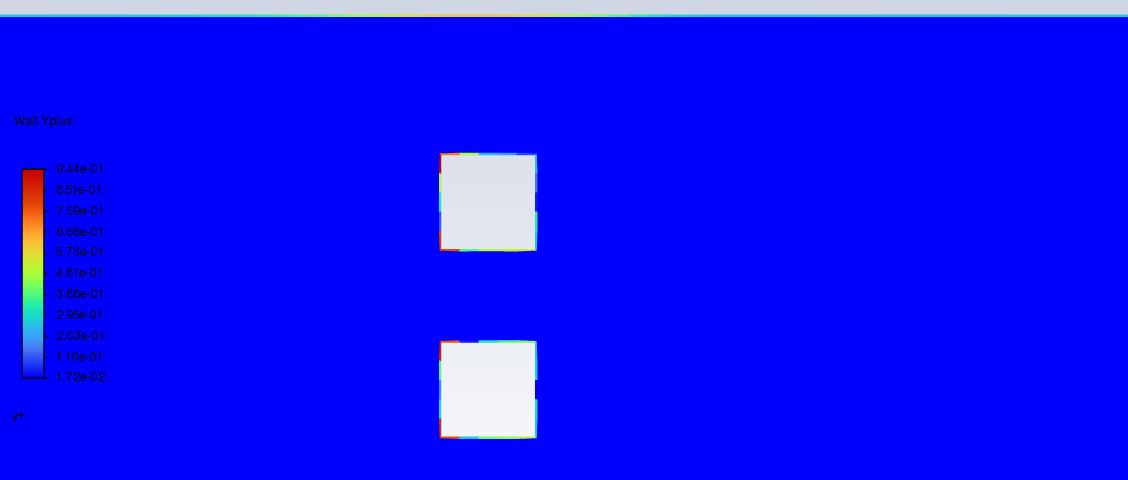
\includegraphics[width=0.7\textwidth]{img/y_plus_k_epsilon_enhanced_wt.png}
    \caption{y+ plot for k-epsilon with enhanced wall treatment}
    \label{fig:k_epsilon_enhanced_y_plus}
\end{figure}

\begin{figure}[h]   
    \centering
    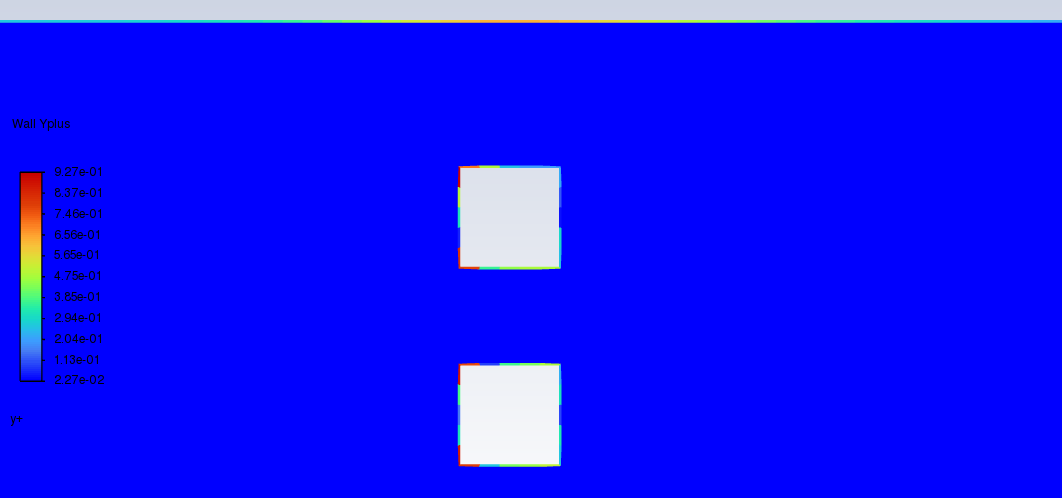
\includegraphics[width=0.7\textwidth]{img/y_plus_k_kl_omega_detail_inf5.png}
    \caption{y+ plot for k-kl-omega}
    \label{fig:k_kl_omega_y_plus}
\end{figure}

\clearpage

For the comparison the basic geometry is used, the meshing is done according to the results of chapter \ref{chapter:meshing}.
To compare the results the velocity, pressure and temperature are plotted.

\paragraph{Temperature Plot}~

The static temperature distribution for all four models is presented in Figure \ref{fig:temp_plot}, with each window labeled for clarity. The laminar model produces the least symmetrical result, contrary to expectations given the geometry. This lack of symmetry appears to stem from eddies that disrupt the flow and cause uneven heat distribution.

The k-epsilon model with enhanced wall treatment shows a sharp temperature gradient immediately after the heaters, leading to a less uniform temperature profile across the outlet. While the outlet temperature matches the other models, the distribution (average across the outlet) is slightly lower.

Both the k-omega and k-kl-omega models deliver more uniform and physically consistent results. The k-kl-omega, while accurate, involves additional equations and computational effort, making it better suited for cases involving transitional flows. k-omega model provides a credible and computationally efficient solution.

\begin{figure}[htbp]   
    \centering
    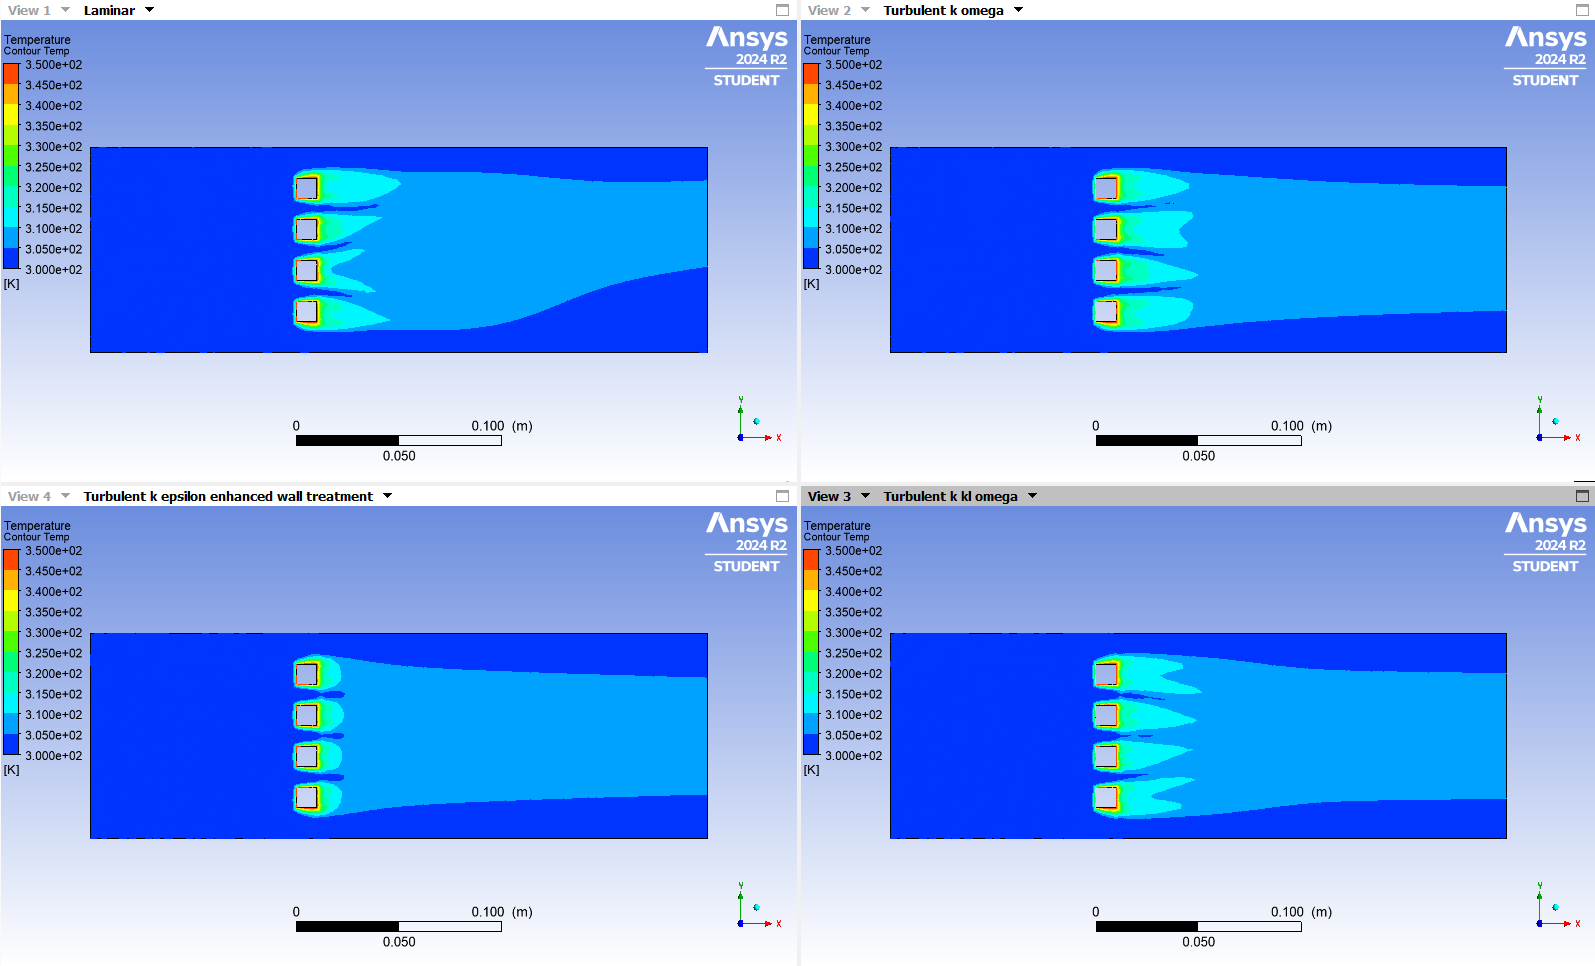
\includegraphics[width=1\textwidth]{img/Temp_plot_comparison.png}
    \caption{Temperature plot for all 4 models}
    \label{fig:temp_plot}
\end{figure}

\paragraph{Velocity Plot}~

The velocity plot supports the observations from the temperature plot.
The velocity distribution in the laminar plot shows smooth transitions near the heating elements with minimal mixing. the k-omega model shows great mixing with well defined recirculation behind the heating element. k-l-omega is quit similar but does not offer the same amount of mixing.
The k-epsilon model shows a well-mixed flow after the heating elements, especially with the enhanced wall treatment the result seems trustworthy.


\begin{figure}[htbp]   
    \centering
    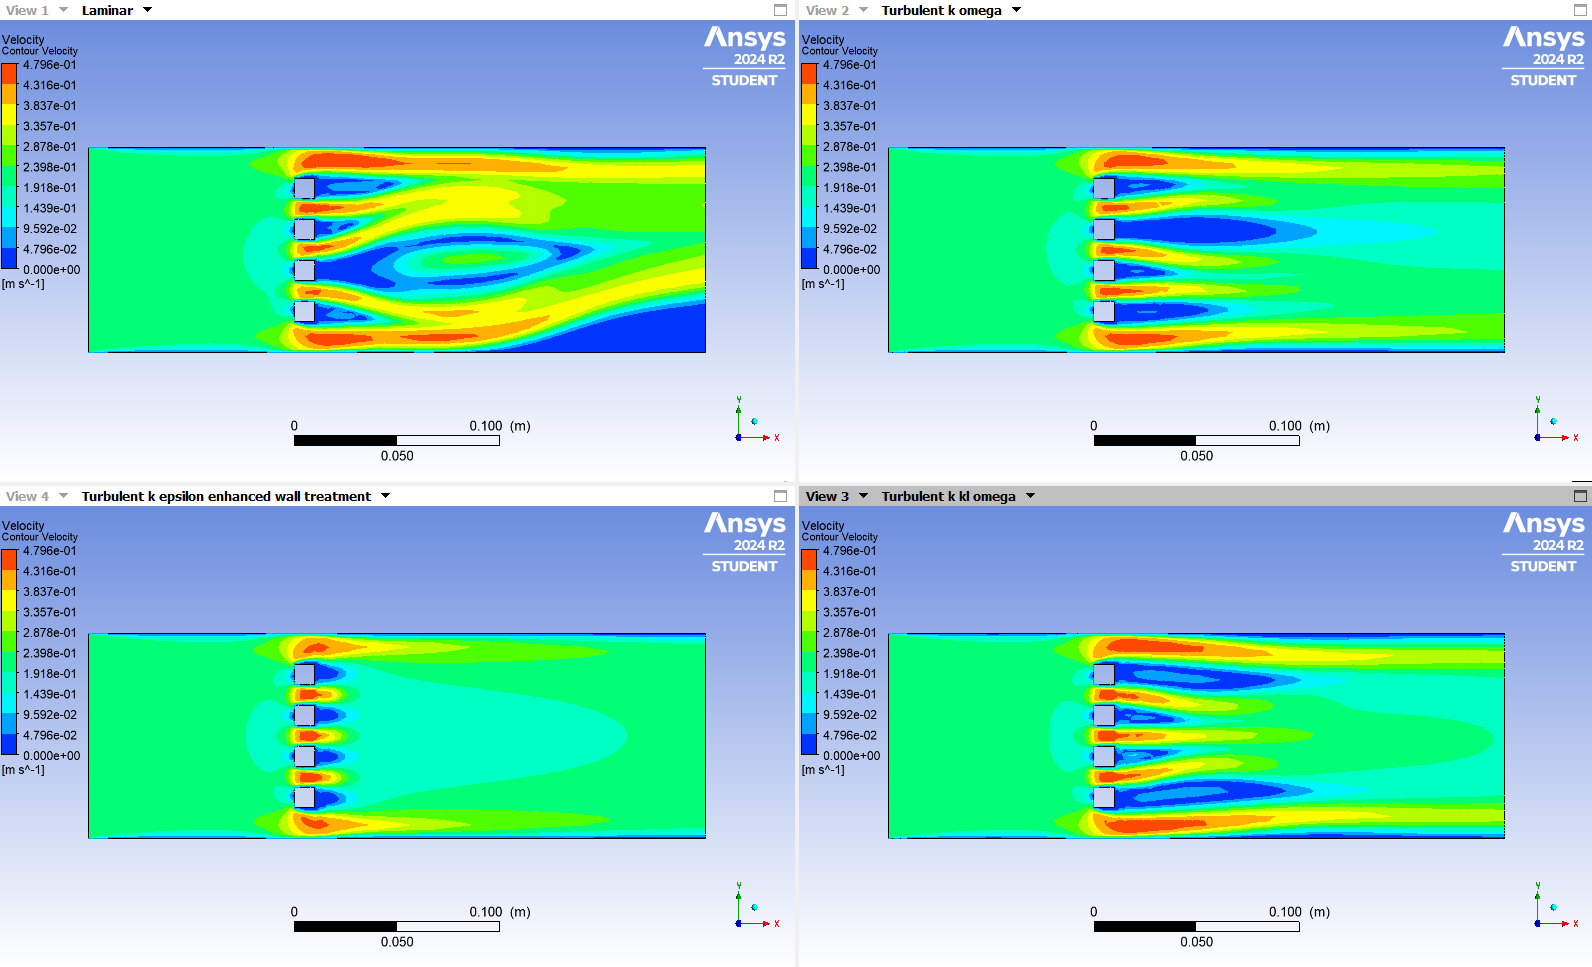
\includegraphics[width=1\textwidth]{img/Velocity_plot_comparison.png}
    \caption{Velocity plot for all 4 models}
    \label{fig:velocity_plot}
\end{figure}

\paragraph{Pressure Plot}~

The velocity and pressure plots are inherently linked through fluid dynamics principles, particularly Bernoulli's equation and the Navier-Stokes equations. In the presented simulations, regions of higher velocity correspond to areas of lower pressure due to the conservation of energy in the flow. This relationship is evident across all turbulence models, where pressure decreases as the flow accelerates past the heaters and recirculation zones are formed.

\begin{figure}[h]   
    \centering
    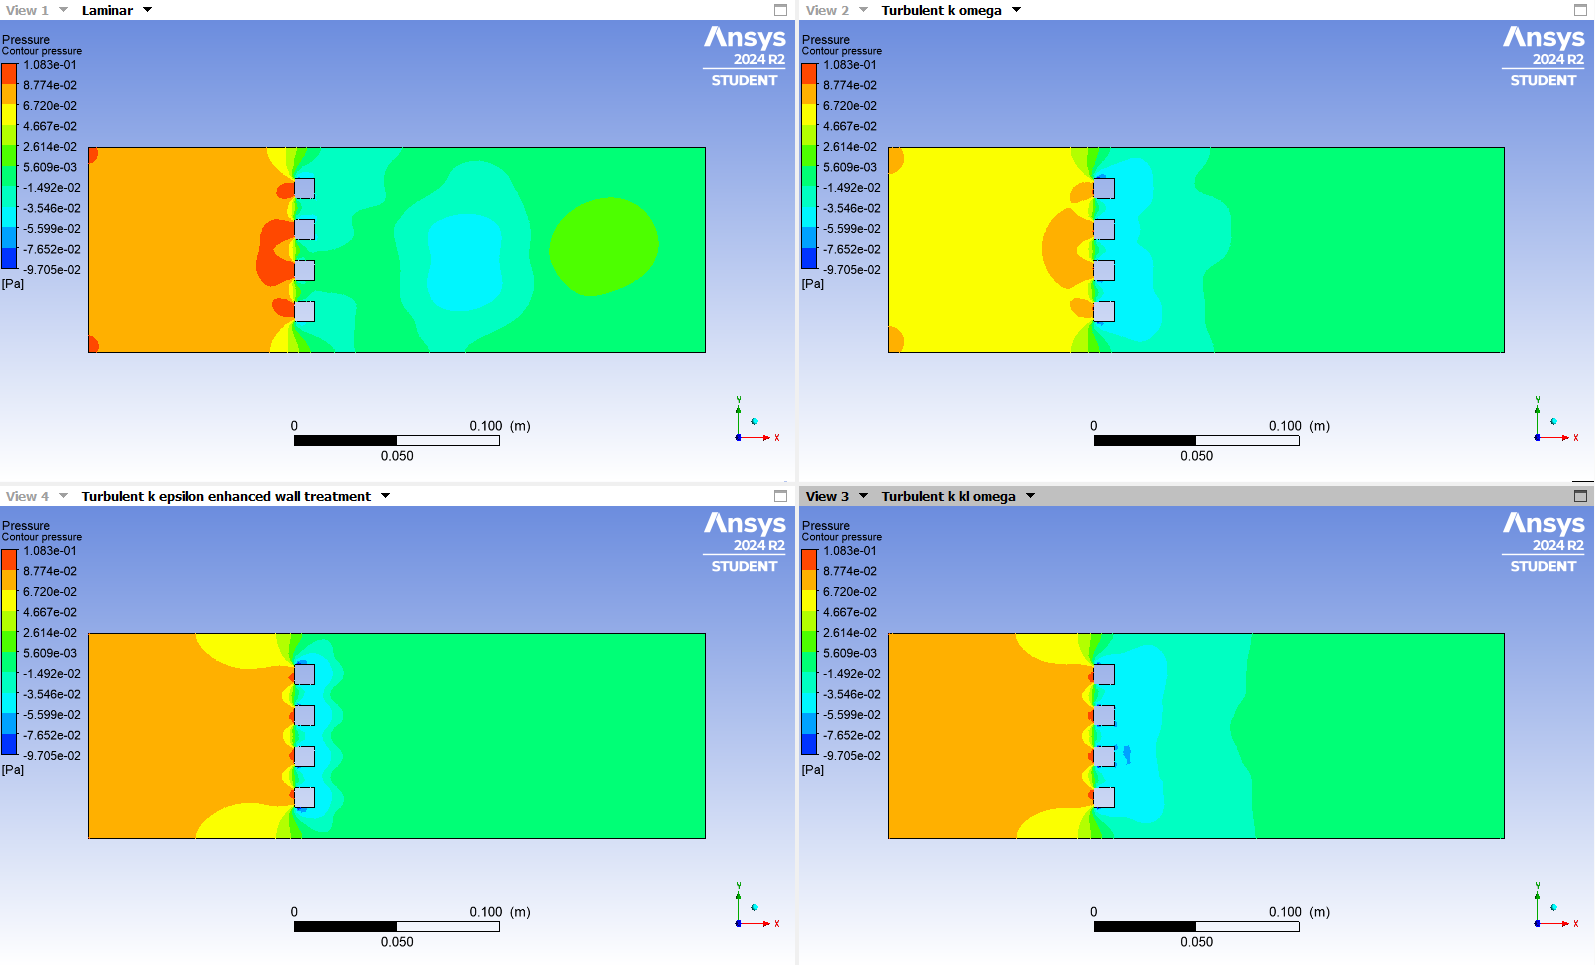
\includegraphics[width=1\textwidth]{img/Pressure_plot_comparison.png}
    \caption{Pressure plot for all 4 models}
    \label{fig:press_plot}
\end{figure}

\paragraph{Chosen Model}~

The k-omega model was chosen for its balance between accuracy and computational efficiency. It provides a credible and symmetrical result for the temperature, velocity, and pressure distributions, aligning well with theoretical expectations and the problem's physical constraints. Unlike the k-kl-omega model, which requires more computational resources due to additional equations, the k-omega model achieves comparable accuracy without the added complexity. This makes it a practical choice for simulations focusing on steady turbulent flow while maintaining reliable performance.


% EOF